\documentclass{beamer} 
\usepackage{tikz}
\usepackage[all]{xy}
\usepackage{amsmath,amssymb}
\usepackage{hyperref}
\usepackage{graphicx}
\usepackage{algorithmic}
\usepackage{multirow}

\DeclareMathOperator*{\argmin}{arg\,min}
\DeclareMathOperator*{\Lik}{Lik}
\DeclareMathOperator*{\PoissonLoss}{PoissonLoss}
\DeclareMathOperator*{\Peaks}{Peaks}
\DeclareMathOperator*{\Segments}{Segments}
\DeclareMathOperator*{\argmax}{arg\,max}
\DeclareMathOperator*{\maximize}{maximize}
\DeclareMathOperator*{\minimize}{minimize}
\newcommand{\sign}{\operatorname{sign}}
\newcommand{\RR}{\mathbb R}
\newcommand{\ZZ}{\mathbb Z}
\newcommand{\NN}{\mathbb N}
\newcommand{\z}{$z = 2, 4, 3, 5, 1$} 

\newcommand{\algo}[1]{\textcolor{#1}{#1}}
\definecolor{PDPA}{HTML}{66C2A5}
\definecolor{CDPA}{HTML}{FC8D62}
\definecolor{GPDPA}{HTML}{4D4D4D}

% Set transparency of non-highlighted sections in the table of
% contents slide.
\setbeamertemplate{section in toc shaded}[default][100]
\AtBeginSection[]
{
  \setbeamercolor{section in toc}{fg=red} 
  \setbeamercolor{section in toc shaded}{fg=black} 
  \begin{frame}
    \tableofcontents[currentsection]
  \end{frame}
}

\begin{document}

\title{Cross-validation for comparing qSIP prediction models trained
  on same or other groups}

\author{
  Toby Dylan Hocking\\
  toby.hocking@nau.edu\\
  toby.hocking@r-project.org\\
}

\maketitle

\begin{frame}
  \frametitle{Motivation and data for predicting growth from genetics}
  \begin{itemize}
  \item Goal: look at past experiments to see which genes influence growth.
  \item Collaboration with Jeff Propster, based on data from Hungate
    et al, mBio (2021), Stone et al, ISME (2023)
  \item Seven past experiments with no omics data, but
    qSIP for total of 188,826 Amplicon Sequence Variants (ASVs),
    including Arizona elevation gradient (experiment=dim),
    \\ Quantitative Microbial Ecology (experiment=qme),
    \\and others (ant, drp, eag, sro, win).
  \item picrust2 (Douglas et al, Nature 2020) infers frequency of 8,380 genes
    in the ASV genome (integer from 0 to 10).
  \item Can we predict a taxon's qSIP growth/activity from its vector of gene frequencies?
    \end{itemize}
% > dim(qsip.dt)                                                                 
% [1] 188826   8407
% > qsip.dt[, .(rows=.N), by=experiment]                                         
%    experiment  rows
% 1:        ant  4046 antartica
% 2:        dim 59067 Dimensions (arizona elevation gradient)
% 3:        drp 16210
% 4:        eag 10761
% 5:        qme 49537 Quantitative Microbial Ecology (alaska/minnesota/arizona/puerto rico)
% 6:        sro 46586
% 7:        win  2619 hopland
\end{frame}

\begin{frame}
  \frametitle{Machine learning predictive analysis of qSIP data}
  \begin{itemize}
  \item Inputs/features $\mathbf x\in\mathbb R^D$ is vector of frequencies for $D=8380$ genes
    (range from 0 to 10).
% !> (gene.tab <- table(as.matrix(gene.dt[1:100])))                               
%      0      1      2      3      4      5      6      7      8      9     10
% 718122 105630  10110   2301    807    362    180    113     87     66    222
%  > gene.range.mat <- sapply(qsip.dt[, gene.names, with=FALSE], range)           
% !> table(gene.range.mat)                                                        
%  gene.range.mat
%     0    1    2    3    4    5    6    7    8    9   10
%  9212 3226 2018  990  510  241  151   81   80   65  186
  \item Output $y\in\mathbb R$ is relative activity/growth per day
    from qSIP (excess atom fraction/EAF normalized by maximum isotope enrichment
    and incubation length, ranging from 0 to 0.3315).
% > range(qsip.dt$growth_per_day)                                                
% [1] 0.0000000 0.3315673
  \item Want to learn $ f(\mathbf x)=y$ (predict growth from genes).
  \item One hypothesis in these data: can learn $f$ on mixed conifer (MC) controls in experiment=dim (room temp), and accurately predict experiment=qme at temp=15C (or vice versa). 
  \item Question: is this expectation consistent with the data?
% There are several experiments that occurred in the same system multiple times. For example, MC (mixed conifer) is the Friends & Foes soil, so comparing qme MC controls and dim MC controls would probably have good prediction accuracy. Note that qme experiment doesn't have "controls" but incubation temperatures of 5 to 35 degrees. The dim experiment was performed at room temperature, so we could compare it to the 15 degree treatment.
  \item Answer by using 10-fold cross-validation: train on one experiment or other, quantify prediction error on test set.
  \end{itemize}
\end{frame}
% > (select.dt <- data.table(site="MC", rbind(                                   
% +   data.table(experiment="dim", treatment="control"),                         
% +   data.table(experiment="qme", treatment="15"))))                            
% site experiment treatment
% 1:   MC        dim   control
% 2:   MC        qme        15
% > dim.qme.controls <- qsip.dt[select.dt, on=.(site,experiment,treatment)]      
% compare <- function(comparison, group.var, DT){                                
% > +   data.table(comparison, group.var, DT=list(DT))                           
% }                                                                              
%   + > comparison.dt <- rbind(                                                    
%   +   compare("controls.between.sites", "site", control.only),                   
%   +   compare("control.vs.carbon.additions", "treatment", qsip.dt[treatment %in%\
%   c("C","CN","control")]),                                                      
%   +   compare("controls.between.experiments", "experiment",dim.qme.controls))    
%   comparison.dt                                                                  
% 1:       controls.between.sites       site <data.table[17225x8407]>
% 2:  control.vs.carbon.additions  treatment <data.table[60877x8407]>
% 3: controls.between.experiments experiment  <data.table[7710x8407]>
% > length(gene.names <- grep("^K", names(qsip.dt), value=TRUE))
% [1] 8380
% > for(comparison.i in 1:nrow(comparison.dt)){
% +   compare.row <- comparison.dt[comparison.i]
% +   print(compare.row$DT[[1]][, .(rows=.N), by=eval(compare.row$group.var)])
% + }
%                 site rows
% 1: glacier_forefield  767
% 2: litchfield_island 1043
% 3:                GL 3560
% 4:                MC 3120
% 5:                PJ 4317
% 6:                PP 4418
%    treatment  rows
% 1:   control 17225
% 2:         C 23214
% 3:        CN 20438

\begin{frame}
  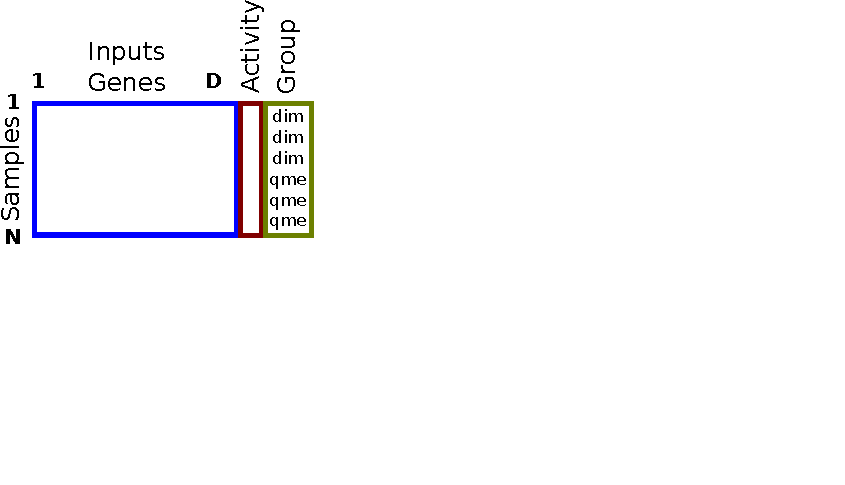
\includegraphics[width=\textwidth]{drawing-cv-same-other-1}
\end{frame}

\begin{frame}
  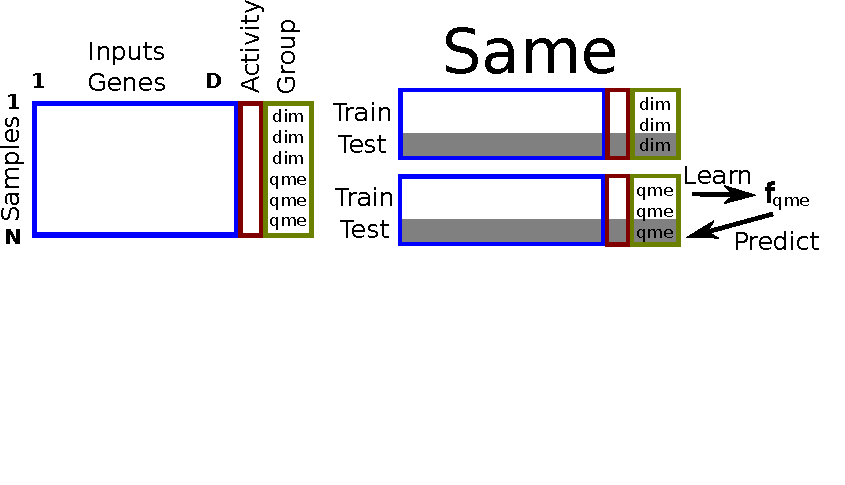
\includegraphics[width=\textwidth]{drawing-cv-same-other-2}
\end{frame}

\begin{frame}
  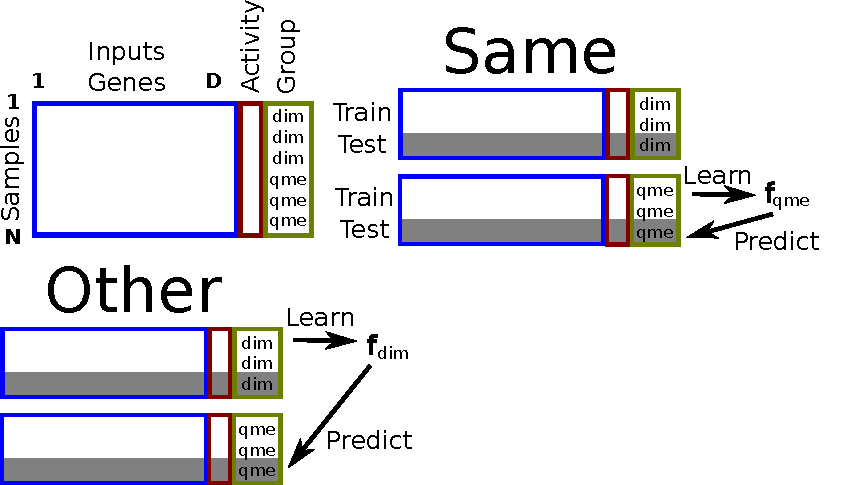
\includegraphics[width=\textwidth]{drawing-cv-same-other-3}
\end{frame}

\begin{frame}
  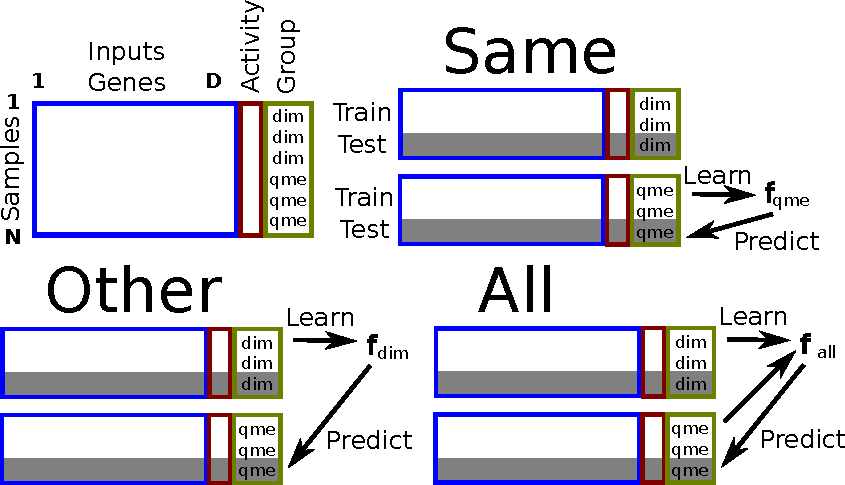
\includegraphics[width=\textwidth]{drawing-cv-same-other-4}
\end{frame}

\begin{frame}
  \frametitle{Comparison 1: controls in different experiments}
  \begin{itemize}
%    experiment rows
% 1:        dim 3120
% 2:        qme 4590
%   comparison.dt                                                                  
% 1:       controls.between.sites       site <data.table[17225x8407]>
% 2:  control.vs.carbon.additions  treatment <data.table[60877x8407]>
% 3: controls.between.experiments experiment  <data.table[7710x8407]>
% > length(gene.names <- grep("^K", names(qsip.dt), value=TRUE))
% [1] 8380
  \item Data table with $N=7710$ rows/observations (ASVs), across two
    experiments dim=3120, qme=4590.
  \item $D=8380$ gene features.
  \item We compare two learning algorithms
    \begin{description}
    \item[cv\_glmnet:] L1 regularized linear model (LASSO), small
      subset of important genes selected and used for prediction
      (other un-important genes are not used for prediction).
    \item[featureless] ignore all genes/features, and always predict
      mean output in train set.
    \end{description}
  \item If there is any non-trivial relationship/pattern learned
    between inputs and outputs, then \textbf{linear model should have
      smaller prediction error than featureless}.
  \item If patterns are similar in different groups/experiments (dim
    and qme), then \textbf{linear model should have similar prediction
      error, when trained on other groups/experiments}.
  \end{itemize}
\end{frame}

\begin{frame}
  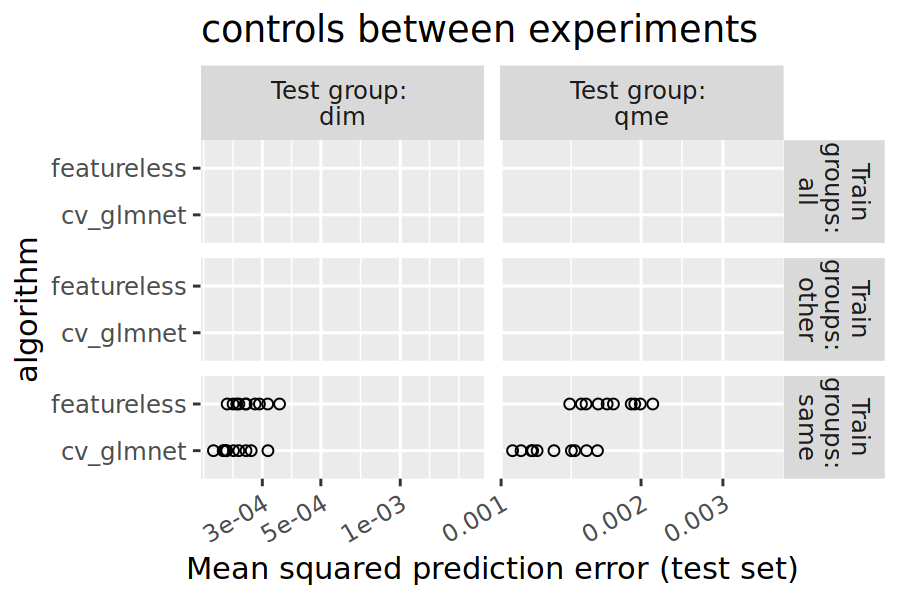
\includegraphics[width=\textwidth]{qsip_pc2_all_new-controls.between.experiments.same.png}
\end{frame}

\begin{frame}
  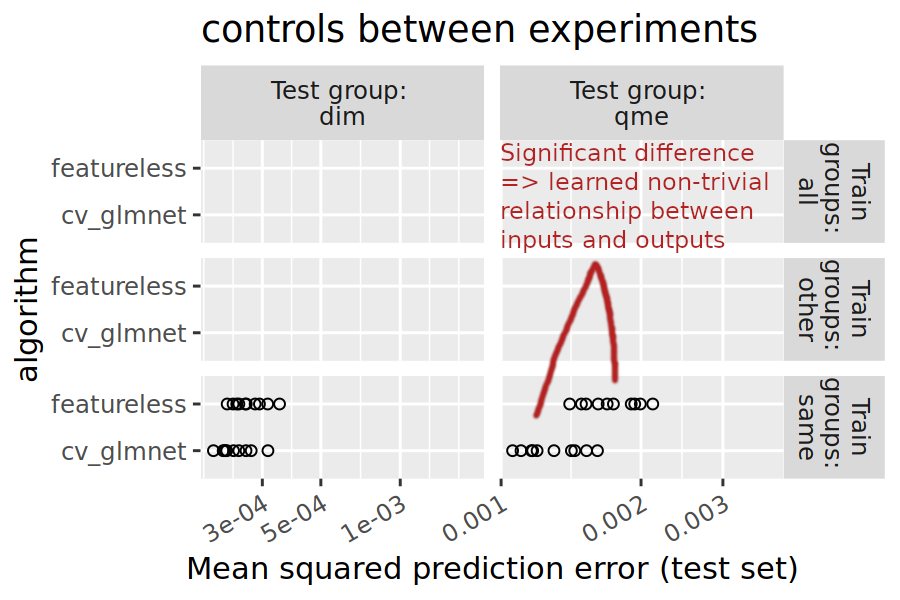
\includegraphics[width=\textwidth]{qsip_pc2_all_new-controls.between.experiments.same.ann.png}
\end{frame}

\begin{frame}
  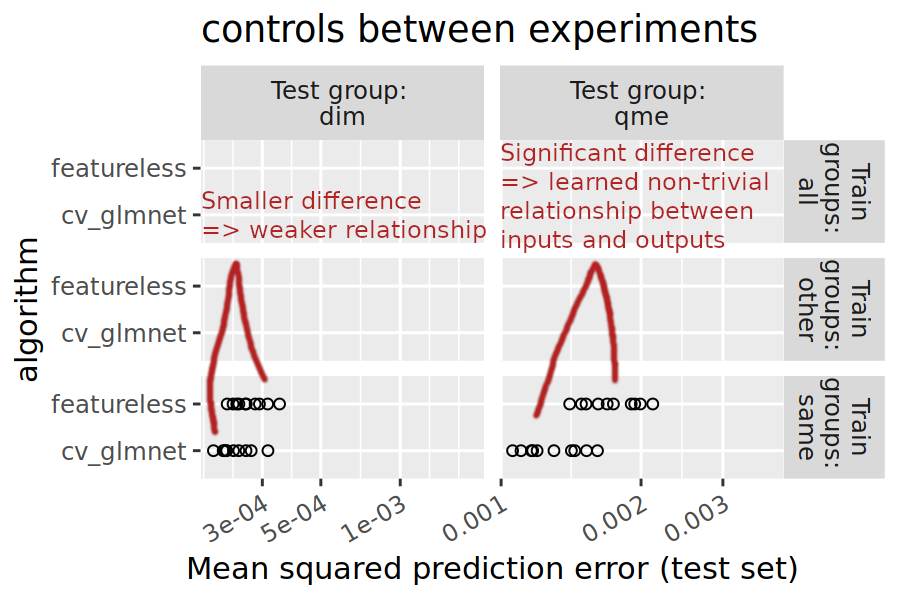
\includegraphics[width=\textwidth]{qsip_pc2_all_new-controls.between.experiments.same.ann2.png}
\end{frame}

\begin{frame}
  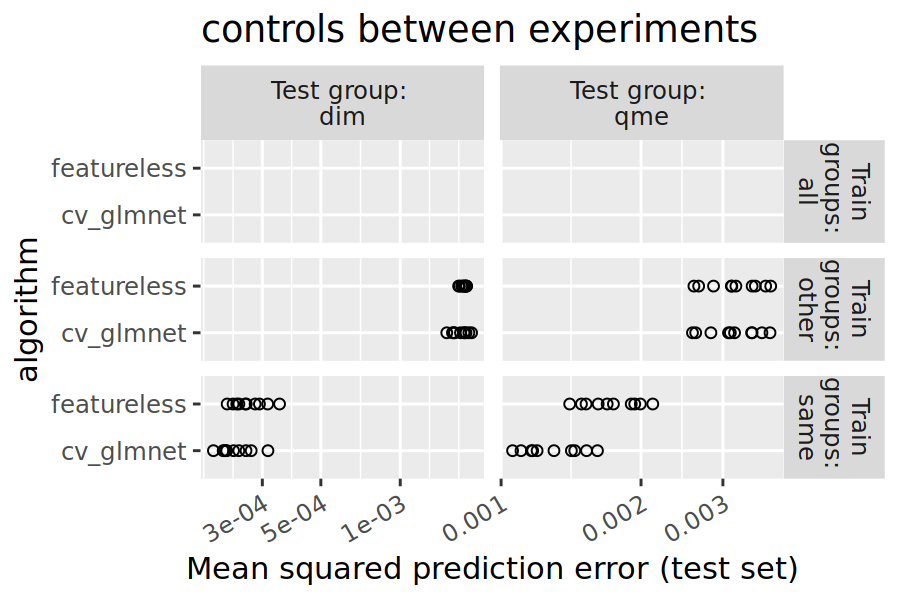
\includegraphics[width=\textwidth]{qsip_pc2_all_new-controls.between.experiments.other.png}
\end{frame}

\begin{frame}
  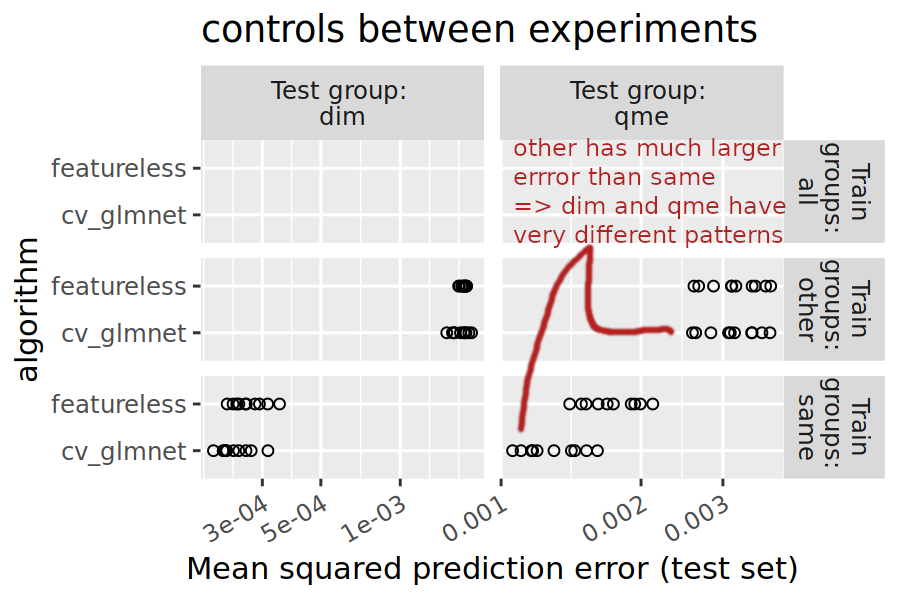
\includegraphics[width=\textwidth]{qsip_pc2_all_new-controls.between.experiments.other.ann.png}
\end{frame}

\begin{frame}
  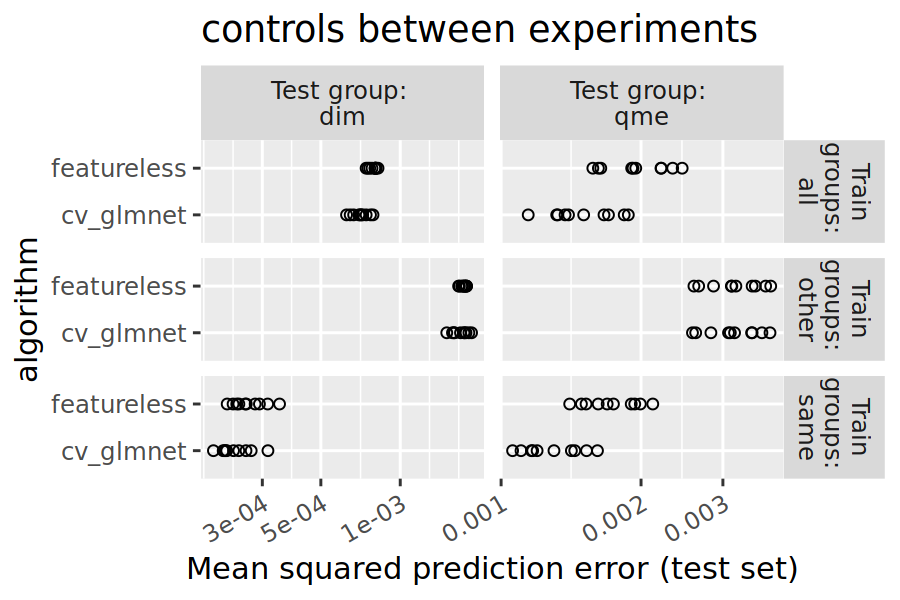
\includegraphics[width=\textwidth]{qsip_pc2_all_new-controls.between.experiments.all.png}
\end{frame}

\begin{frame}
    \frametitle{Interpretation of linear model prediction error and weights}
    \begin{itemize}
    \item Hypothesis was: expect we can learn $f$ on mixed conifer (MC) controls in experiment=dim (room temp), and accurately predict experiment=qme at temp=15C (or vice versa). 
    \item Prediction error cross-validation analysis on previous slide is not consistent with that hypothesis.
    \item So there should be a different prediction function in each
      experiment. What is the difference?
    \item The L1 regularized linear model (LASSO) can be interpreted
      in terms of which genes are important/used for prediction
      (non-zero weights/coefficients) and others are ignored
      (weights=0, not used for prediction).
    \item Compute and plot weights which are non-zero/important in all 10
      train/test splits of cross-validation.
    \end{itemize}
\end{frame}

\begin{frame}
  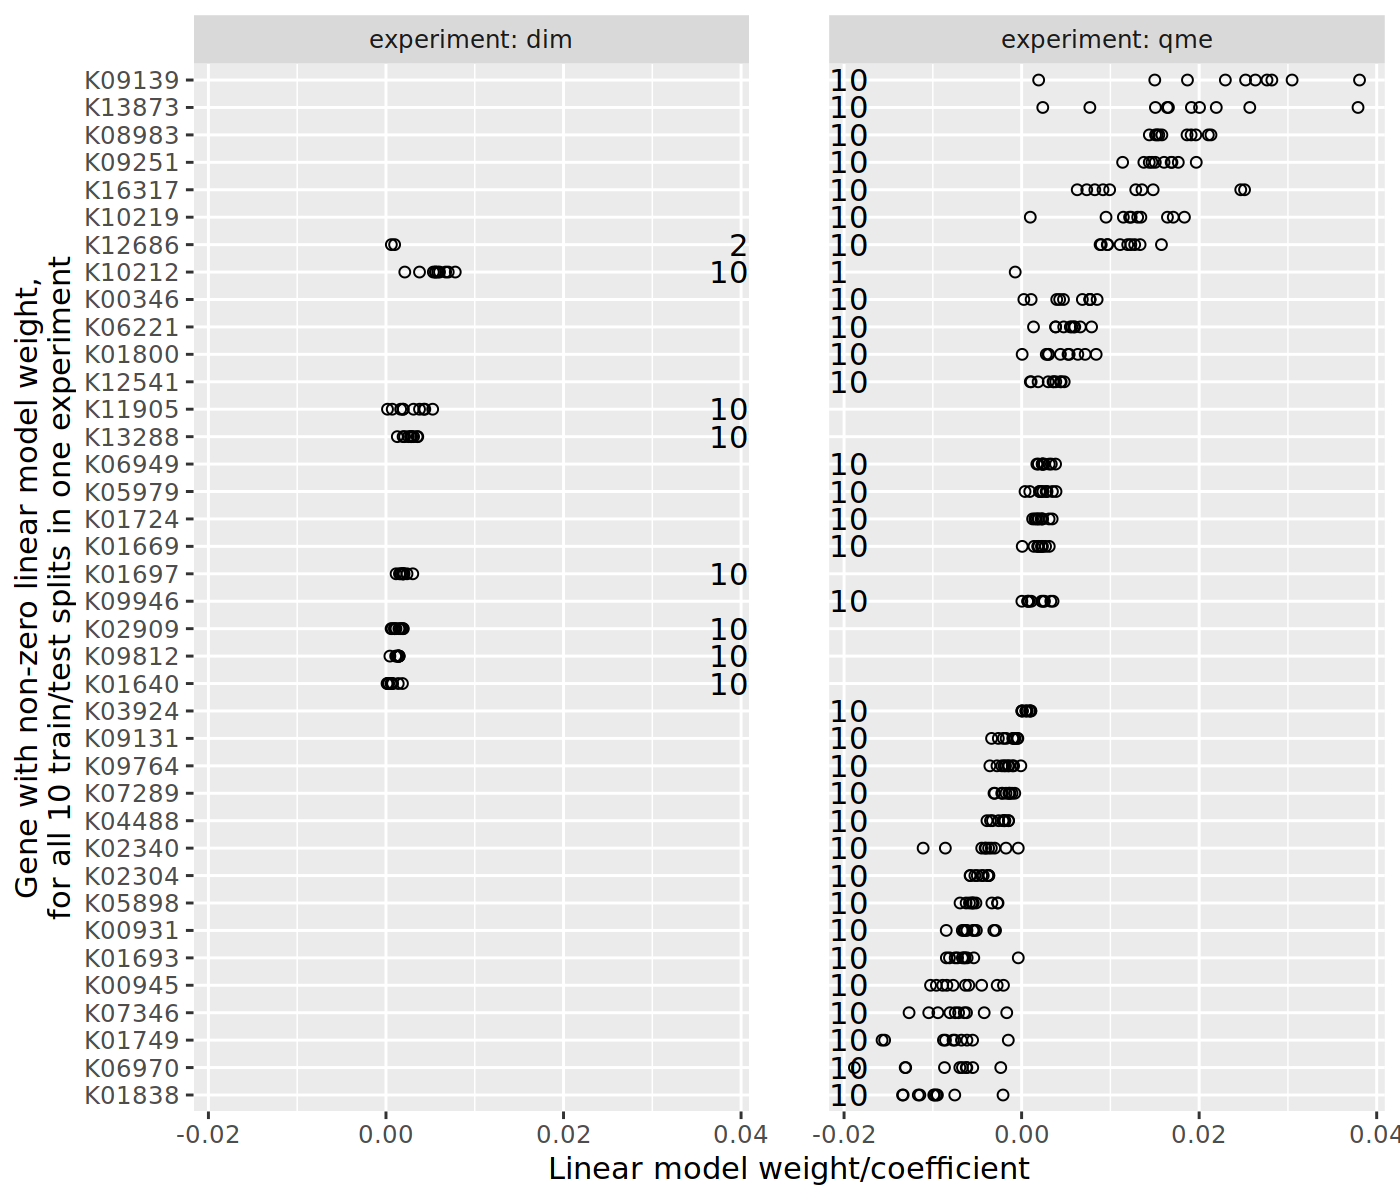
\includegraphics[width=\textwidth]{2024-01-09-qsip_pc2_all_new-controls.between.experiments.weights.png}
\end{frame}

%   comparison.dt                                                                  
% 1:       controls.between.sites       site <data.table[17225x8407]>
% 2:  control.vs.carbon.additions  treatment <data.table[60877x8407]>
% 3: controls.between.experiments experiment  <data.table[7710x8407]>
% > length(gene.names <- grep("^K", names(qsip.dt), value=TRUE))
% [1] 8380
%    treatment  rows
% 1:   control 17225
% 2:         C 23214
% 3:        CN 20438

\begin{frame}
  \frametitle{Comparison 2: control versus carbon additions}
  \begin{itemize}
  \item $N=60877$ samples total, in 3 groups/treatments:
    control=17225, C=23214 (carbon added), CN=20438 (carbon and nitrogen added).
  \item Same $D=8380$ gene features.
  \item Can we train on one group/treatment, and predict accurately on another?
  \end{itemize}
\end{frame}

\begin{frame}
  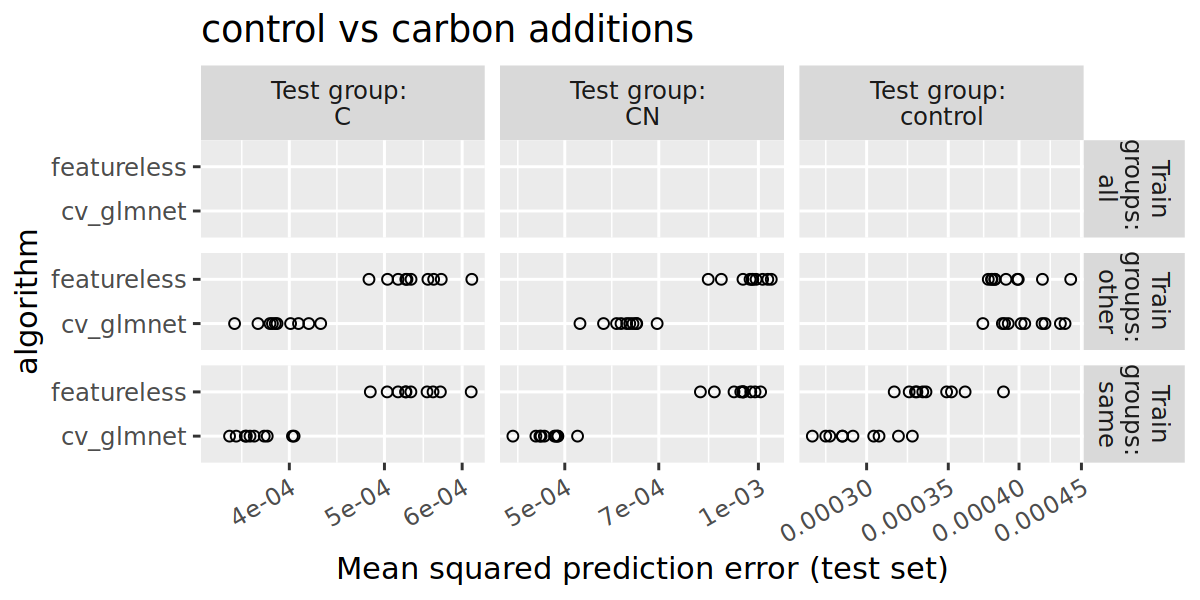
\includegraphics[width=\textwidth]{qsip_pc2_all_new-control.vs.carbon.additions.other.png}
\end{frame}

\begin{frame}
  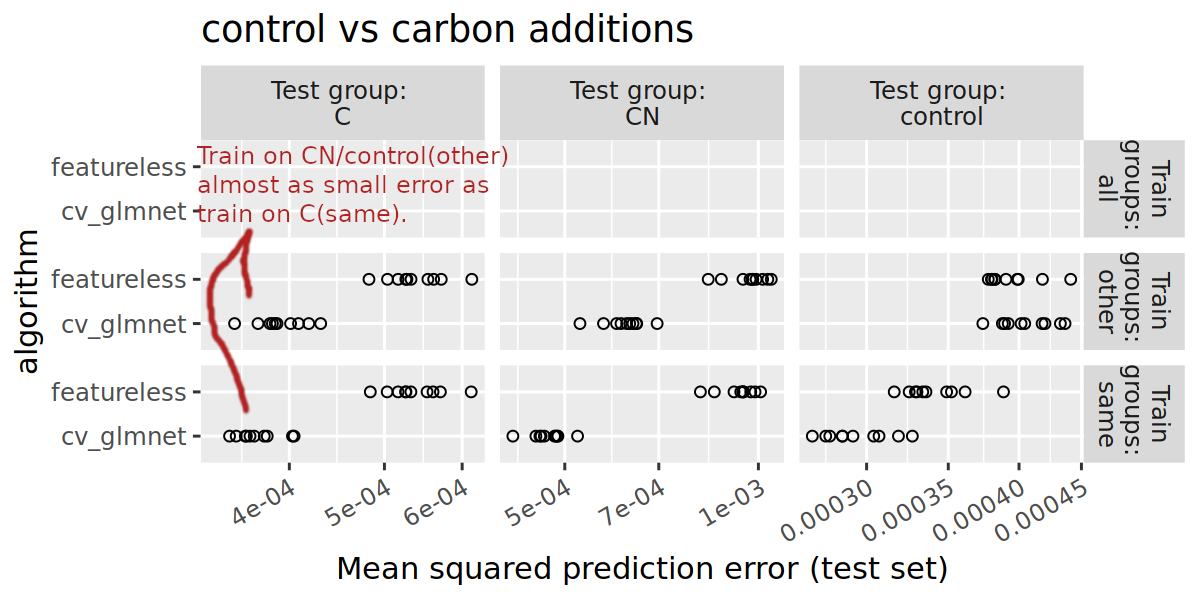
\includegraphics[width=\textwidth]{qsip_pc2_all_new-control.vs.carbon.additions.other.1.png}
\end{frame}

\begin{frame}
  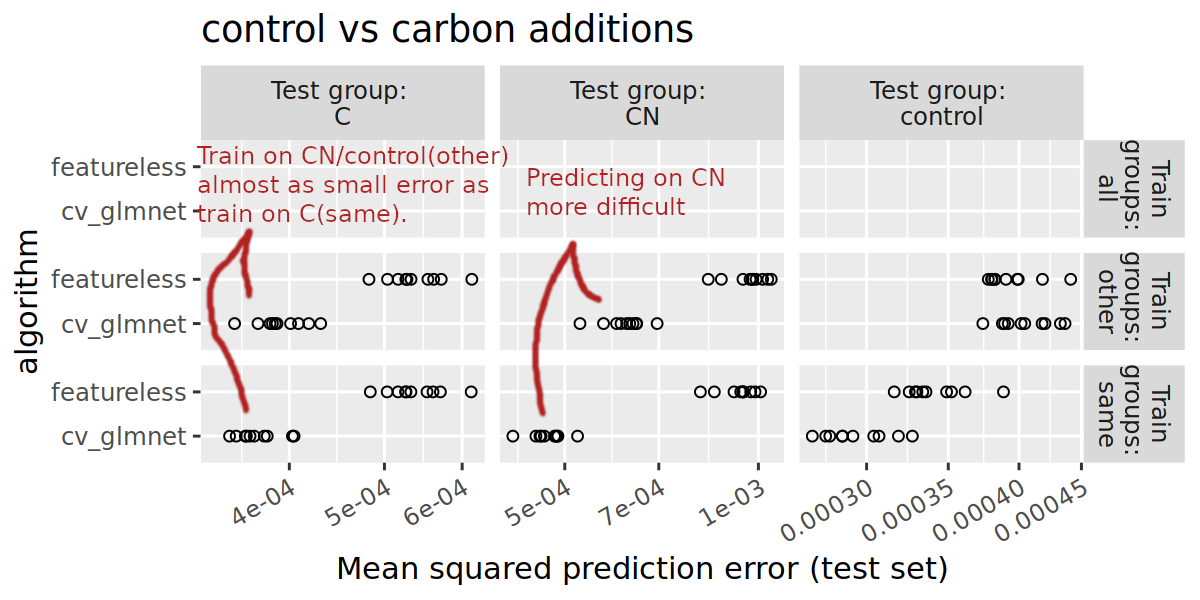
\includegraphics[width=\textwidth]{qsip_pc2_all_new-control.vs.carbon.additions.other.2.png}
\end{frame}

\begin{frame}
  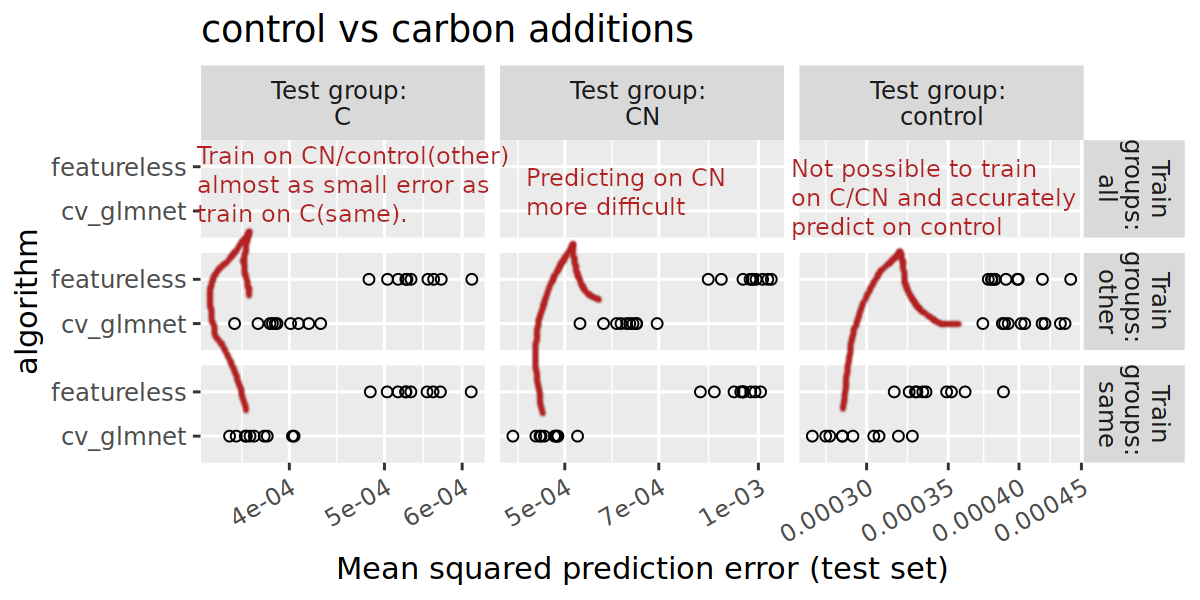
\includegraphics[width=\textwidth]{qsip_pc2_all_new-control.vs.carbon.additions.other.3.png}
\end{frame}

% I think comparing controls to carbon additions (C, CN, detritus, rhizo, cellulose, etc.) would be interesting and would likely have bad prediction accuracy. We are also interested in differences across systems, so comparing controls between sites would be great, too.


\begin{frame}
  \frametitle{Discussion and conclusions}
  \begin{itemize}
  \item Often we want to know if we have similar or different patterns
    in different data groups (train on one experiment/treatment, predict
    on another).
  \item Cross-validation can be used to determine the extent to which
    we can train on one group, and accurately predict on another.
  \item Machine learning algorithms like L1 regularized linear models
    (LASSO/cv\_glmnet) are additionally interpretable in terms of which features
    are used for prediction (can be compared between models trained on
    different groups).
  \item Free/open-source software available: mlr3resampling R package
    on CRAN and \url{https://github.com/tdhock/mlr3resampling}
  \item Let's collaborate! Contact: toby.hocking@nau.edu, toby.hocking@r-project.org
  \end{itemize}
\end{frame}

\end{document}